\documentclass[11pt,a4paper]{article}
\usepackage[spanish,es-nodecimaldot]{babel}	% Utilizar español
\usepackage[utf8]{inputenc}					% Caracteres UTF-8
\usepackage{graphicx}						% Imagenes
\usepackage[hidelinks]{hyperref}			% Poner enlaces sin marcarlos en rojo
\usepackage{fancyhdr}						% Modificar encabezados y pies de pagina
\usepackage{float}							% Insertar figuras
\usepackage[textwidth=390pt]{geometry}		% Anchura de la pagina
\usepackage[nottoc]{tocbibind}				% Referencias (no incluir num pagina indice en Indice)
\usepackage{enumitem}						% Permitir enumerate con distintos simbolos
\usepackage[T1]{fontenc}					% Usar textsc en sections
\usepackage{amsmath}						% Símbolos matemáticos
\usepackage{listings}
\usepackage{color}

 
\definecolor{codegreen}{rgb}{0,0.6,0}
\definecolor{codegray}{rgb}{0.5,0.5,0.5}
\definecolor{codepurple}{rgb}{0.58,0,0.82}
\definecolor{backcolour}{rgb}{0.99,0.99,0.99}
 
\lstdefinestyle{mystyle}{
    backgroundcolor=\color{backcolour},   
    commentstyle=\color{codegreen},
    keywordstyle=\color{magenta},
    numberstyle=\tiny\color{codegray},
    stringstyle=\color{codepurple},
    basicstyle=\footnotesize,
    breakatwhitespace=false,         
    breaklines=true,                 
    captionpos=b,                    
    keepspaces=true,                 
    numbers=left,                    
    numbersep=5pt,                  
    showspaces=false,                
    showstringspaces=false,
    showtabs=false,                  
    tabsize=2
}
 
\lstset{style=mystyle, language=Python}

% Comando para poner el nombre de la asignatura
\newcommand{\asignatura}{Visión por Computador}
\newcommand{\autor}{José María Sánchez Guerrero}
\newcommand{\titulo}{Cuestionario 3}
\newcommand{\subtitulo}{Feature Matching y Panoramas}

% Configuracion de encabezados y pies de pagina
\pagestyle{fancy}
\lhead{\autor{}}
\rhead{\asignatura{}}
\lfoot{Grado en Ingeniería Informática}
\cfoot{}
\rfoot{\thepage}
\renewcommand{\headrulewidth}{0.4pt}		% Linea cabeza de pagina
\renewcommand{\footrulewidth}{0.4pt}		% Linea pie de pagina

\begin{document}
\pagenumbering{gobble}

% Pagina de titulo
\begin{titlepage}

\begin{minipage}{\textwidth}

\centering

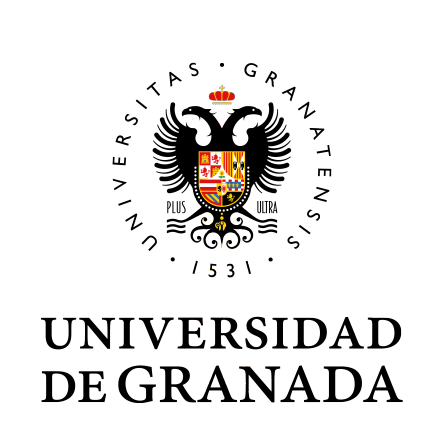
\includegraphics[scale=0.5]{img/ugr.png}\\

\textsc{\Large \asignatura{}\\[0.2cm]}
\textsc{GRADO EN INGENIERÍA INFORMÁTICA}\\[1cm]

\noindent\rule[-1ex]{\textwidth}{1pt}\\[1.5ex]
\textsc{{\Huge \titulo\\[0.5ex]}}
\textsc{{\Large \subtitulo\\}}
\noindent\rule[-1ex]{\textwidth}{2pt}\\[3.5ex]

\end{minipage}

\vspace{0.5cm}

\begin{minipage}{\textwidth}

\centering

\textbf{Autor}\\ {\autor{}}\\[2.5ex]
\textbf{Rama}\\ {Computación y Sistemas Inteligentes}\\[2.5ex]
\vspace{0.3cm}


\includegraphics[scale=0.3]{img/etsiit.jpeg}

\vspace{0.7cm}
\textsc{Escuela Técnica Superior de Ingenierías Informática y de Telecomunicación}\\
\vspace{1cm}
\textsc{Curso 2019-2020}
\end{minipage}
\end{titlepage}

\pagenumbering{arabic}
\tableofcontents
\thispagestyle{empty}				% No usar estilo en la pagina de indice

\newpage

\setlength{\parskip}{1em}


\section*{Ejercicio 1}
\addcontentsline{toc}{section}{Ejercicio 1}
\textbf{¿Cuál es la transformación más fuerte de la geometría de una escena que puede introducirse al tomar una foto de ella? Dar algún ejemplo.}

Es la \textbf{proyección}, porque es la transformación que menos propiedades de la imagen preserva. Cambia tanto el paralelismo, como las dimensiones,
o los ángulos. Un ejemplo de ello lo podemos ver en el siguiente cubo (todas artistas y ángulos miden lo mismo):
\begin{figure}[H]
\centering
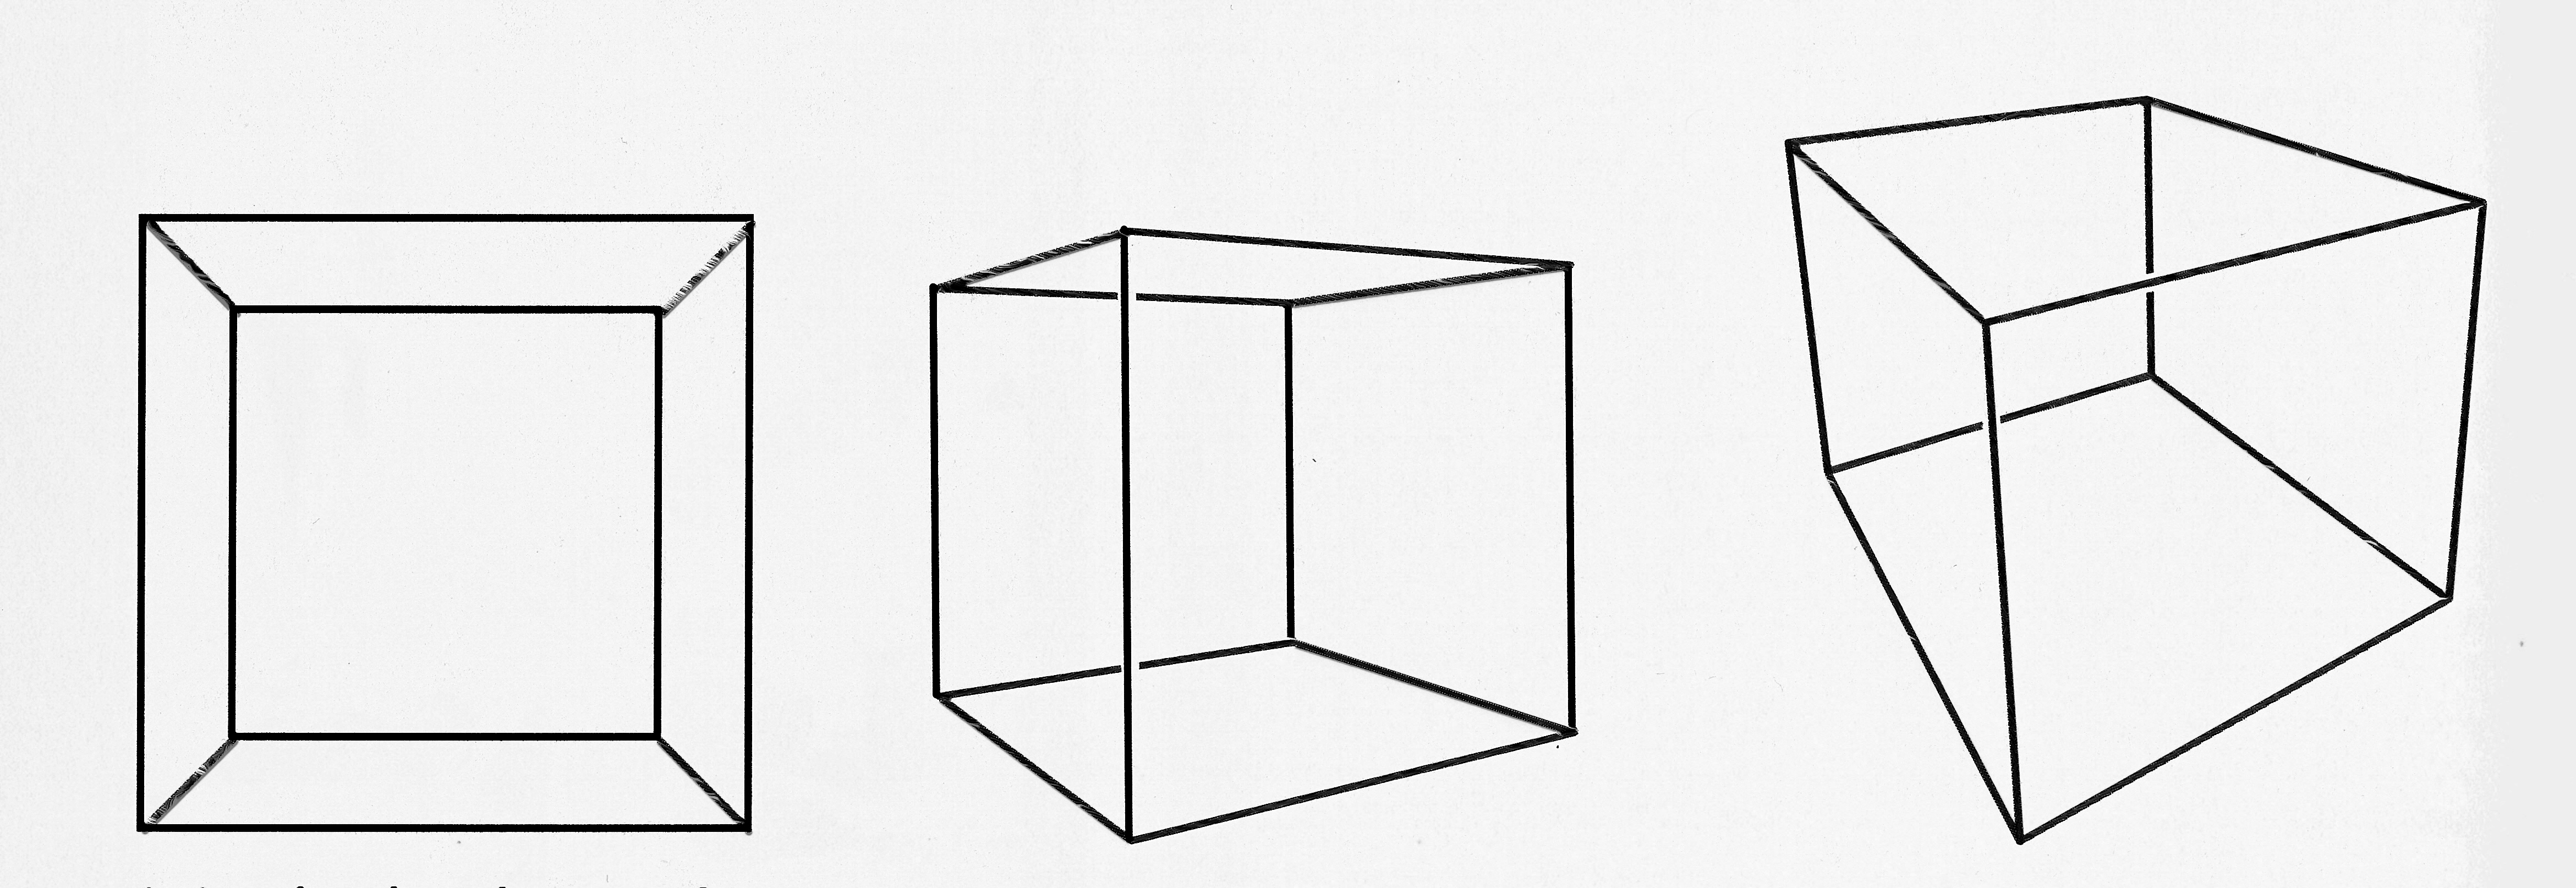
\includegraphics[scale=0.6]{img/cubo.jpg}
\end{figure}

En la imagen de la izquierda podemos ver cómo la cara frontal si conserva los 90º en sus ángulos y si proyectamos sus líneas paralelas al infinito
nunca se cruzarán, pero ya vemos cómo las aristas frontales y posteriores no miden lo mismo, cuando si son iguales. En los demás cubos vemos cómo
ningun ángulo se mantiene con 90º y si proyectamos dos líneas paralelas cualesquiera hasta el infinito, terminarán cruzándose. 



\section*{Ejercicio 2}
\addcontentsline{toc}{section}{Ejercicio 2}
\textbf{¿Por qué es necesario usar el plano proyectivo para estudiar las transformaciones en las imágenes de fotos de escenas? Dar algún ejemplo.}

Porque pese a que no se conserven tamaños o ángulos, si conserva las relaciones de \textbf{incidencia}, es decir, todos los puntos que pertenecen a
una línea, seguirán perteneciendo a esta después de la transformación.

Y de \textbf{cross-ratio}, la cual dice que, dados 4 puntos A, B, C y D pertenecientes a una recta, su \textit{cross-ratio} es igual a $(A,B;C,D)=
(AC\cdot{BD})/(BC\cdot{AD})$. Por ejemplo, si lo llevamos a un plano proyectivo como el siguiente:
\begin{figure}[H]
\centering
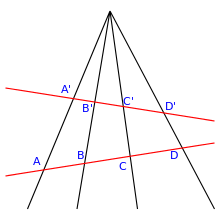
\includegraphics[scale=0.6]{img/plano-proyectivo.jpg}
\end{figure}

Los puntos A, B, C, D y A', B', C', D' están relacionados porque sus relaciones cruzadas, (A, B; C, D) y (A', B'; C', D') son iguales.



\section*{Ejercicio 3}
\addcontentsline{toc}{section}{Ejercicio 3}
\textbf{Sabemos que en el plano proyectivo un punto no existe en el sentido del plano afín, sino que se define por una clase de equivalencia de
vectores definida por $\{k(x,y,1),k\neq{0}\}$. Razone usando las coordenadas proyectivas de los puntos afines de una recta que pase por el (0,0)
del plano afín y verifique que los puntos de la recta del infinito del plano proyectivo son necesariamente vectores del tipo (*,*,0) con *=cualquier
número.}

Si tenemos en cuenta que *=cualquier número, por ejemplo $a$, cualquier punto representado en el plano proyectivo vendría dado por:
\begin{equation*}
(ax, ay, 1) = (x,y,\frac{1}{a})
\end{equation*}
Un punto en el infinito del plano proyectivo hace que $a=\infty$ y en consecuencia que $\frac{1}{a} = 0$, y por tanto podemos decir que su vector de
coordenadas es del tipo $(x,y,0)$.



\section*{Ejercicio 4}
\addcontentsline{toc}{section}{Ejercicio 4}
\textbf{¿Qué propiedades de la geometría de un plano quedan invariantes cuando se toma una foto de él? Justificar la respuesta.}

Dependiendo de la foto que hayamos tomado, las propiedades que quedan invariantes serán unas u otras. Si tomamos la siguiente imagen de las
transparencias como guía, las transformaciones que no se producen son la de su misma fila más las que aparecen debajo:
\begin{figure}[H]
\centering
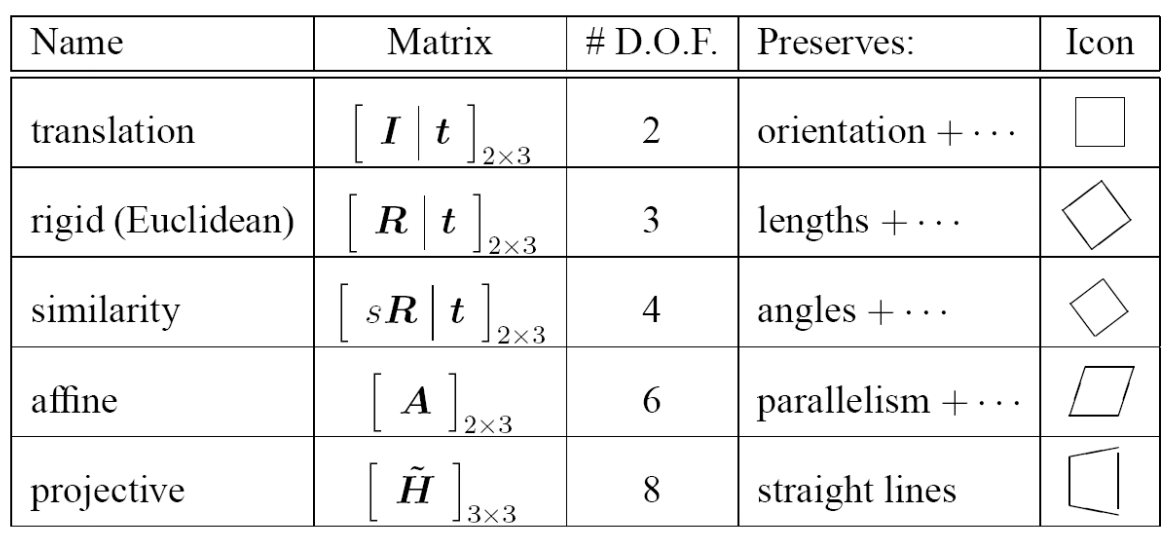
\includegraphics[scale=0.4]{img/transformaciones.png}
\end{figure}

Por ejemplo, teniendo en cuenta las fotografía de abajo, si tomamos la de la izquierda, vemos cómo la foto no ha sufrido cambios y las propiedades
que se conservan son la orientación + tamaños + ... + líneas rectas. Mientras que si tomamos la imagen de la derecha, que es una foto en el plano
proyectivo, sólo conserva las propiedades de éste (como pueden ser la incidencia o el \textit{cross-ratio} comentados en el ejercicio 2).
\begin{figure}[H]
\centering
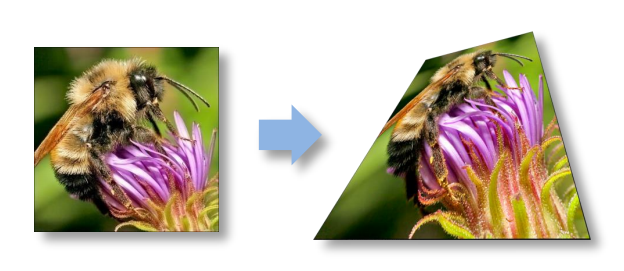
\includegraphics[scale=0.6]{img/transformaciones2.png}
\end{figure}



\section*{Ejercicio 5}
\addcontentsline{toc}{section}{Ejercicio 5}
\textbf{En coordenadas homogéneas los puntos y rectas del plano se representan por vectores de tres coordenadas (notados x y l respectivamente), de
manera que si una recta contiene a un punto se verifica la ecuación $x^Tl=0$, es decir $(x_1,x_2,x_3)\begin{pmatrix}a\\b\\c\end{pmatrix} = 0$.
Considere una homografía H que transforma vectores de puntos, $x' = Hx$. Dado que una homografía transforma vectores de tres coordenadas también
existen homografías G para transformar vectores de rectas $l' = Gl$. Suponga una recta $l$ y un punto $x$ que verifican $x^Tl=0$ en el plano proyectivo
y suponga que conoce una homografía H que transforma vectores de puntos. En estas condiciones ¿cuál es la homografía G que transforma los vectores de
las rectas? Deducirla matemáticamente.}

Para calcular una homografía G tal que $l'=Gl$, tendremos en cuenta que para todos los puntos de la recta $l$, si aplicamos una homografía conocida H
($x'=Hx$) obtenemos una nueva recta $l'$. Si cada punto $x'$ debe de estar contenido en la recta $l'$, podemos verificar que $(x')^Tl'=0$.

Si ahora consideramos las transformaciones que realizan las homografías H y G en los vectores de puntos y rectas, respectivamente, tenemos que:
\begin{equation*}
(x')^Tl' = (Hx)^T Gl = x^T H^T Gl = 0
\end{equation*}

Por otra parte, si hacemos que $H^TG=I$, siendo I la matriz identidad, podremos llegar a donde queríamos:
\begin{equation*}
x^T H^T Gl = x^T (H^T G) l = x^T (I) l = x^T l = 0
\end{equation*}

Por último, ya sólo nos queda despejar la G de forma que:
\begin{equation*}
H^T G = I \rightarrow G = (H^-1)^T
\end{equation*}

\section*{Ejercicio 6}
\addcontentsline{toc}{section}{Ejercicio 6}
\textbf{¿Cuál es el mínimo número de escalares necesarios para fijar una homografía general? ¿Y si la homografía es afín? Justificar la respuesta}

El número mínimo de escalares es 8, porque en una homografía general G, definida como $G = \begin{bmatrix}a & b & c\\d & e & f \\g & h & 1\end{bmatrix}$,
vemos que la última variable siempre valdrá 1.

En cuanto a una homografía afin, los grados de libertad mínimos que tenemos son 6, ya que la última fila de la matriz anterior valdrá (0,0,1).

Tanto una como otra vienen bastante bien explicadas y con ejemplos en el siguiente artículo:

https://courses.cs.washington.edu/courses/csep576/11sp/pdf/Transformations.pdf


\section*{Ejercicio 7}
\addcontentsline{toc}{section}{Ejercicio 7}
\textbf{Defina una homografía entre planos proyectivos que haga que el punto (3,0,2) del plano proyectivo-1 se transforme en un punto de la recta del
infinito del plano proyectivo-2? Justificar la respuesta.}

Tenemos que calcular una homografía H, definida como una matriz 3x3, tal que la multiplicación de ésta con el punto dado, se convierta en un punto de
la recta del infinito del plano proyectivo-2, es decir:
\begin{equation*}
\begin{bmatrix}a & b & c\\d & e & f \\g & h & 1\end{bmatrix}\cdot \begin{bmatrix}3\\0\\2\end{bmatrix} = \begin{bmatrix}x'\\y'\\w'\end{bmatrix}
\end{equation*}

El sistema de ecuaciones resultante es el siguiente:
\begin{equation*}\left\{\begin{matrix}
x' = 3a+0b+2c\\ 
y' = 3d+0e+2f\\ 
w' = 3g+0h+(2\cdot 1)
\end{matrix}\right.\end{equation*}

Como ya sabemos que es un punto de la recta del infinito, $w'$ tendrá que valer 0. Si sustituimos en la última ecuación tenemos que:
$$w' = 3g+0h+(2\cdot1)$$
$$0  = 3g+0+2$$
$$g = -(3/2)$$

Por lo tanto, si cuando aplicamos una homografía entre planos proyectivos hacemos que el valor $g$ de la matriz valga $-(3/2)$, nos aseguramos que el
punto (3,0,2) será un punto de la recta del infinito del plano proyectivo 2.


\section*{Ejercicio 8}
\addcontentsline{toc}{section}{Ejercicio 8}
\textbf{Una homografía general $\mathbf{H}=\begin{pmatrix}a & b & c \\ d & e & f \\
g & h & i \end{pmatrix} = \begin{bmatrix} \mathbf{A} & \mathbf{t} \\ \mathbf{v}^T & v
\end{bmatrix}$, $\text{det}(\mathbf{H}) \neq 0$ admite una
descomposición única en movimiento elementales de la siguiente
forma $\mathbf{H} = \mathbf{H}_S\mathbf{H}_A\mathbf{H}_P$ donde $\mathbf{H}_S$
representa la homografía de una similaridad
(escala, giro y traslación), $\mathbf{H}_A$ la homografía de un movimiento afín
puro y $\mathbf{H}_P$ una transformación proyectiva pura. Es decir,}

$$\mathbf{H}_S = \begin{pmatrix} s\cos\theta & -s\sin\theta & t_x \\ s\sin\theta & s\cos\theta & t_y \\
0 & 0 & 1 \end{pmatrix} \equiv \begin{bmatrix} s\mathbf{R} & \mathbf{t} \\ \mathbf{0}^T & 1 \end{bmatrix}, s>0$$

$$\mathbf{H}_A = \begin{pmatrix} a & c & 0 \\ 0 & b &0 \\ 0 & 0 & 1 \end{pmatrix} \equiv
\begin{bmatrix} s\mathbf{K} & \mathbf{0} \\ \mathbf{0}^T & 1 \end{bmatrix}, \text{det}(\mathbf{K}=1$$

$$\mathbf{H}_P = \begin{pmatrix} 1 & 0 & 0 \\ 0 & 1 &0 \\ v_1 & v_2 & v \end{pmatrix} \equiv
\begin{bmatrix} \mathbf{I} & \mathbf{0} \\ \mathbf{v}^T & v \end{bmatrix}, v \neq 0$$

(Notación: en negrita son vectores o matrices)

Describir un algoritmo que permite encontrar las matrices de la
descomposición de una matriz $\mathbf{H}$ dada. Aplicarlo para encontrar la
descomposición de

$$
  \mathbf{H} = \begin{pmatrix}
  1.707 & 0.586 & 1.0 \\
  2.707 & 8.242 & 2.0 \\
  1.0 & 2.0 & 1.0
  \end{pmatrix}
$$



\section*{Ejercicio 9}
\addcontentsline{toc}{section}{Ejercicio 9}
\textbf{¿Cuáles son las propiedades necesarias y suficientes para que una matriz defina un movimiento geométrico no degenerado entre planos? Justificar
la respuesta}

Para definir un movimiento geométrico no degenerado entre planos, tenemos que transformar un punto de un plano $P$ a un punto de otro plano $P'$. Sin embargo,
esta transformación también la podremos hacer desde $P'$ hasta $P$, lo que quiere decir que una de las propiedades tiene que ser la \textbf{inversa}. Su
matriz debe aceptar que pasemos de $M \rightarrow M^{-1}$, o lo que es lo mismo, que su determinante sea igual a 0.

La otra propiedad necesaria es que la matriz de la transformación tiene que ser de \textbf{3x3}, ya que los planos están definidos en 3 dimensiones.
Para transformar un punto del plano con 3 coordenadas, necesitamos una matriz 3x3 para así multiplicarlas y obtener un punto de la misma dimensión.


\section*{Ejercicio 10}
\addcontentsline{toc}{section}{Ejercicio 10}
\textbf{¿Qué información de la imagen usa el detector de Harris para seleccionar puntos? ¿El detector de Harris detecta patrones geométricos o fotométricos?
Justificar la contestación.}

Mediante una ventana deslizante, el detector de Harris va recorriendo la imagen y buscando los cambios más bruscos en la intensidad del gradiente. Una vez
hemos obtenido estos puntos, utilizamos el criterio de Harris para ver con cuáles nos quedaremos o no:
$$ M' = det(M) - k(Traza(M))^2 $$

Los píxeles que tengan un valor alto (utilizando un umbral determinado), serán los puntos Harris elegidos.

Harris detecta tanto patrones geométricos cómo fotométricos, ya que utliza la geometría para poder detectar, por ejemplo las esquinas; y los fotométricos,
porque como acabamos de comentar, también se hace uso de la intensidad del gradiente.


\section*{Ejercicio 11}
\addcontentsline{toc}{section}{Ejercicio 11}
\textbf{¿Sería adecuado usar como descriptor de un punto Harris los valores de los píxeles de su región de soporte? Identifique ventajas, inconvenientes y
mecanismos de superación de estos últimos.}

No encuentro ninguna ventaja, ya que estamos hablando de los descriptores. Es cierto que el detector si es invariante a la rotación o cambios de intensidad,
sin embargo, el descriptor no (Harris te va a detectar los mismos puntos).

Los inconvenientes que tiene esto es que las sombras, los cambios de intensidades de luz, etc. sí que cambian los valores de los píxeles, haciendo que dos
descriptores sean distintos teniendo que ser iguales. Para solucionarlo, podemos utilizar los descriptores SIFT, que crea una ventana de 16x16 y calcula un
histograma con las orientaciones de los gradientes para cada uno sus cuadrantes 4x4. De esta forma, no sólo tenemos en cuenta uno de los gradientes, sino
un vecindario de ellos.


\section*{Ejercicio 12}
\addcontentsline{toc}{section}{Ejercicio 12}
\textbf{Describa un par de criterios que sirvan para seleccionar parejas de puntos en correspondencias (“matching”) a partir de descriptores de regiones
extraídos de dos imágenes. ¿Por qué no es posible garantizar que todas las parejas son correctas?}

Vamos a describir los dos métodos utilizados en las prácticas:
\begin{itemize}
	\item \textbf{Brute Force}. Comprueba punto a punto la distancia (por ejemplo Euclídea) que existe entre el primer y segundo descriptor, y posteriormente,
		  selecciona la correspondencia que obtenga el valor más bajo. Este método es bastante simple, pero no podemos garantizar que todas las parejas sean
		  correctas, ya que si tenemos objetos parecidos en la imagen o que sigan patrones, se puede confundir.
	\item \textbf{Lowe Average 2NN}. Este clasificador de vecino más cercano encuentra las k mejores coincidencias para cada descriptor. El parámetro k=2, ya
		  que es un 2NN, y entre estos nos quedaremos con uno siguiendo el método de Lowe. Este método elige el mejor match $m$ sii $m < umbral * m2$, siendo $m2$
		  la distancia hasta el match $m$. De esta forma, con más de un descriptor, evitamos el problema anterior de las correspondencias asociadas.
\end{itemize}


\section*{Ejercicio 13}
\addcontentsline{toc}{section}{Ejercicio 13}
\textbf{Cual es el objetivo principal del uso de la técnica RANSAC en el cálculo de una homografía. Justificar la respuesta}

El objetivo principal es realizar un ajuste únicamente de los puntos válidos ($inliers$), descartando los puntos atípicos ($outliers$). Esto lo hacemos para
realizar un ajuste bueno cuando hagamos la homografía, y que no nos perjudique el ruido o una mala interpretación en los datos.

Vamos a ver un ejemplo de cómo RANSAC ajusta la siguiente recta comprobando que la distancia entre los $inliers$ y los $outliers$ supera un umbral y, en
consecuencia, descartando estos últimos.
\begin{figure}[H]
\centering
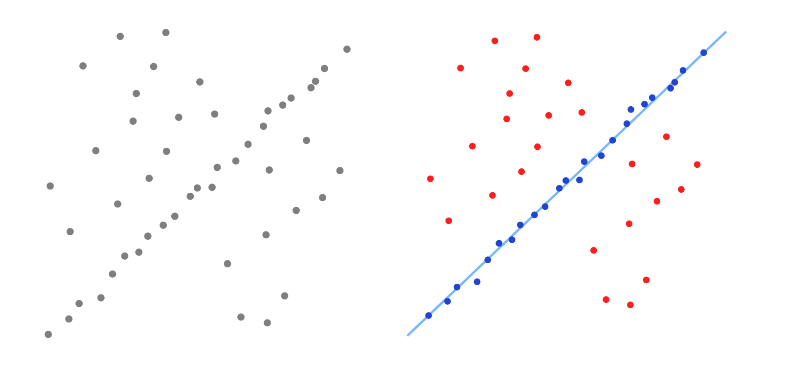
\includegraphics[scale=0.6]{img/ransac.png}
\end{figure}


\section*{Ejercicio 14}
\addcontentsline{toc}{section}{Ejercicio 14}
\textbf{Si tengo 4 imágenes de una escena de manera que se solapan la 1-2, 2-3 y 3-4. ¿Cuál es el número mínimo de parejas de puntos en correspondencias
necesarios para montar un mosaico? Justificar la respuesta}

El número mínimo de puntos necesarios para realizar una homografía son 4 parejas de puntos en correspondencias (2 matches). Si queremos hacer un mosaico de 4
imágenes, tendremos que realizar 3 homografías, por lo que necesitaremos 12 parejas de puntos en correspondencia.


\section*{Ejercicio 15}
\addcontentsline{toc}{section}{Ejercicio 15}
\textbf{¿En la confección de un mosaico con proyección rectangular es esperable que aparezcan deformaciones geométricas de la escena real? ¿Cuáles y por qué?
¿Bajo qué condiciones esas deformaciones podrían no estar presentes? Justificar la respuesta.}

Si es esperable que aparezcan deformaciones, ya que está todo proyectado en el mismo plano pero cada una de las imágenes tomadas tiene una dirección diferente.

Las deformaciones que se generan son debidas a las propias proyección de la imagen en el mismo plano. Otra deformación generada es la que obtenemos entre imagen
e imagen, es decir, a medida que nos vamos alejando de la imagen central, el error en el mosaico aumenta (por eso solemos empezar desde la central).

No obtendríamos estas deformaciones si proyectasemos en un cilindro, en el cual no se deforma la escena. No obstante, si produciría una pequeña distorsión debido
a la propia representación en forma cilíndrica.  Por ejemplo, lo podemos observar en los caminos de la siguiente imagen:
\begin{figure}[H]
\centering
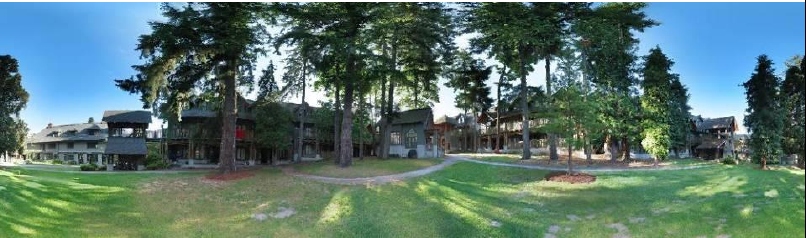
\includegraphics[scale=0.6]{img/casa.png}
\end{figure}

\end{document}